\documentclass{article}
\usepackage[margin=1in]{geometry}
\usepackage{graphicx}
\usepackage{hyperref}
\graphicspath{ {images/} }

\begin{document}

\section*{Windowing}
\subsection*{Why we use windowing?}
When you use the FFT to convert a signal from the time domain to the time-frequency domain you are basing it on a finite number of samples.

\begin{itemize}
	\item FFT is based on a finite number of samples
	\item FFT assumes that sample is one period of a periodic signal
	\item when there are an integer number of periods in the sample this works out very nicely and data matches FFT's assumption.
	\begin{itemize}
		\item this usually is not the case :(
		\item we use window functions to reduce the aliasing this causes
		\item the finiteness of the measured signal may result in a truncated waveform
	\end{itemize}
	\item when number of periods in the sample is not an integer its endpoints are discontinuous
	\item artificial discontinuities show up in FFT as high frequency aliasing not found in original signal
	\begin{itemize}
		\item aliasing is often FAR higher than the nyquist limit
	\end{itemize}
	\item Spectrum the FFT returns is smeared
	\begin{itemize}
		\item energy from one frequency appears to leak over into neighboring frequencies
		\item \textit{called spectral leakage}
	\end{itemize}
\end{itemize}
\textbf{Windowing helps minimize the effects of performing an FFT over a noninteger number of cycles!}

\subsection*{Basic idea of windowing}
\begin{itemize}
	\item windowing reduces the amplitudes of the samples at the boundaries of the period
	\item the idea is this reduces the aliasing of the artificial discontinuities in the FFT
	\item windows generally approach zero towards their edges
	\item windows general have a single maxima at the center
\end{itemize}

\subsection*{Considerations when windowing}
\textit{was tired when writing this so it needs editing!} \\

Windowing of a sample waveform i.e. $cos(\omega t)$ causes its Fourier transform to develop non-zero values (spectral leakage) at frequencies other than $\omega$. This interferance tends to be greatest at frequencies near $\omega$ and decreases as you get farther from $\omega$. \\

This becomes more of a problem when you have multiple waveforms in the same sample that are dissimilar and one component is weaker than the others. Leakage from the stronger component can obscure the weaker frequency's presence. A rectangular window is good for sinusoids of comparable strength, but it is a poor choice for sinusoids of disparate amplitudes. This is sometimes described as sinusoids with a low-dynamic-range.

On the other end of the spectrum windows with the poorest resolution and sensitivity. These can reveal relatively weak sinusoids in the presence of additive random noise. That is because noise produces a stronger response with hidh-dynamic-range windows than with high-resolution windows. Therefore, high-dynamic range windows are often justified in wideband applications where the spectrum being analyzed is expected to contain components of various amplitudes.

In between are moderate windows, such as the Hamming and Hann windows. 

\subsection*{General Types}
\subsubsection*{Low-Dynamic-Range Windows}
\begin{itemize}
	\item rectangular window is good for sinusoids of comparable strength
	\item poor results with sinusoids of disparate amplitudes
	\item low dynamic range
\end{itemize}

\subsubsection*{High-Dynamic-Range Windows}
\begin{itemize}
	\item these are used in wide-band applications. spectrum being analyzed contains many different components of various amplitudes.
	\item reveal relatively weak sinusoids in the presence of additive random noise.
	\item noise produces a stronger response with high-dynamic-range windows than with high-resolution windows.
\end{itemize}

\subsubsection*{When selecting a type of window function}
\textit{todo: indepth analysis of types of window functions}
\begin{itemize}
	\item in general the Hanning (Hann) window is satisfactory in almost all cases
	\begin{itemize}
		\item has good frequency resolution
		\item reduced spectral leakage \\
			\textit{the tendency for energy in one frequency to appear to smear into neighboring frequencies}
	\end{itemize}
	\item if 
\end{itemize}

\subsubsection*{Moderate Windows}
\textit{such as hamming and Hann windows}
\begin{itemize}
	\item commonly used in narrowband applications
	\item tradeoff between components of similar strengths and frequencies and disimilar strengths and frequencies
\end{itemize}

\subsection*{Window Functions}
\subsubsection*{B-Spline window: Rectangular Window}
This is the simplest window. it makes it appaear as though the wave form simply turns on and off.
$$w(n) = 1$$
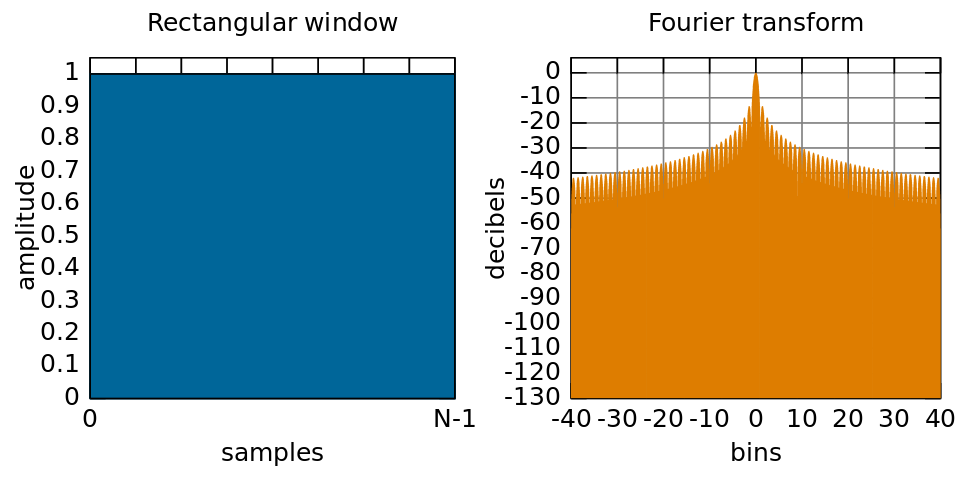
\includegraphics[width=4in]{images/rectangular-window.png}


\subsubsection*{B-Spline Window: Triangular WIndow}
$$w(n) = 1 - |\frac{n - \frac{N - 1}{2}}{\frac{L}{2}}|$$

\subsection*{Hann (Hanning Window)}
$$w(n) = 0.5(1 - cos(\frac{2\pi n}{N - 1})) = hav(\frac{2 \pi n}{N - 1})$$ \\
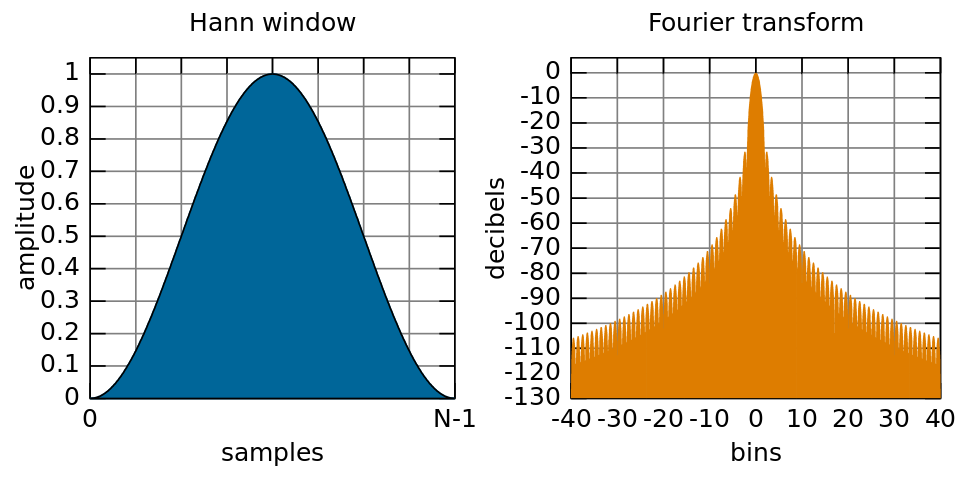
\includegraphics[width=4in]{images/hann-window.png}

\subsection*{Hamming Window}
Te window is optimized to minimize the maximum (nearest) side lobe, giving it a height of about one-fifth that of the Hann window.
$$w(n) = \alpha - \beta cos(\frac{2\pi n}{N - 1})$$
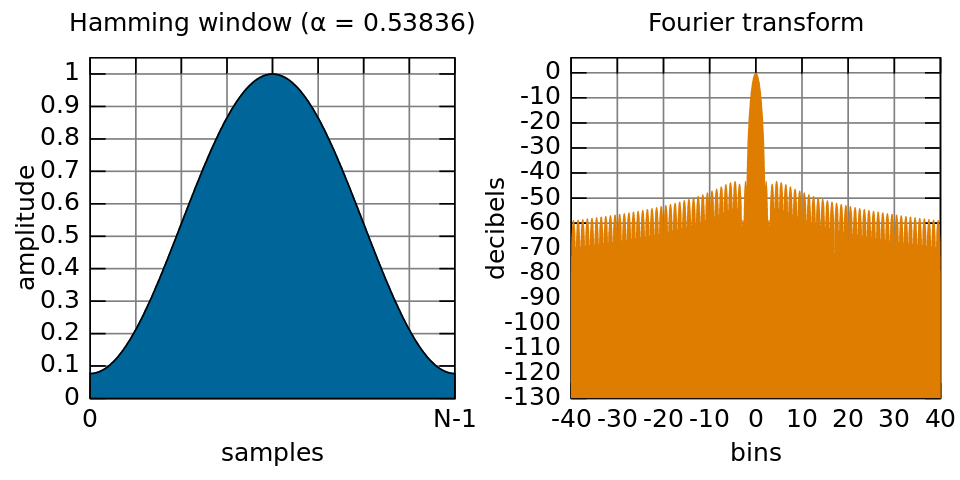
\includegraphics[width=4in]{images/hamming-window.png}


\section*{Sources}
\url{http://www.ni.com/white-paper/4844/en/} \\
\url{https://en.wikipedia.org/wiki/Window_function} \\
\url{https://en.wikipedia.org/wiki/Hann_function} \\

\end{document}